% Preamble: \usepackage{pgfplots} \pgfplotsset{compat=1.18}
\begin{figure}[htbp]
\centering
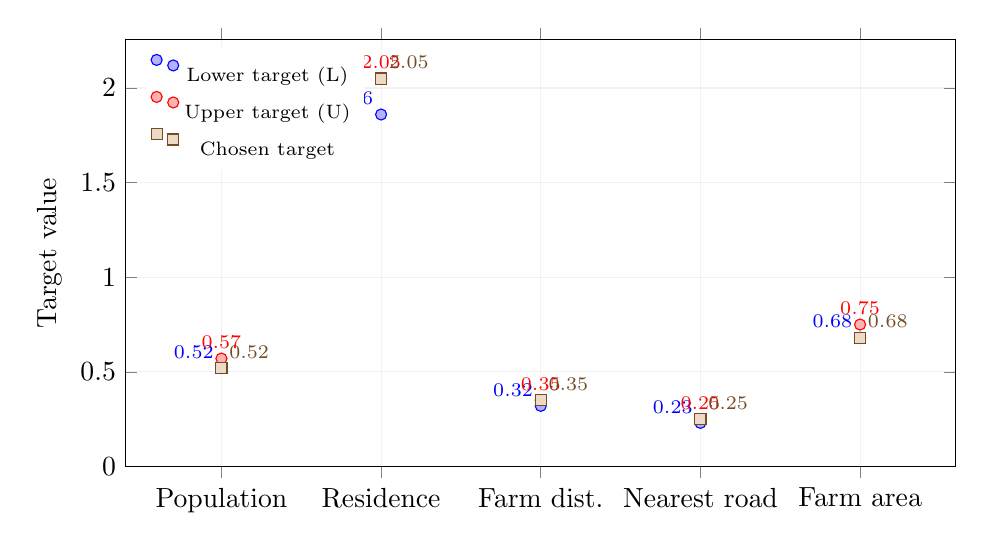
\begin{tikzpicture}
\begin{axis}[
  ybar=0pt,
  width=\textwidth, height=7cm,
  xtick=data,
  xticklabels={Population, Residence, Farm dist., Nearest road, Farm area},
  ylabel={Target value},
  ymin=0, enlarge x limits=0.15,
  grid=both, grid style={opacity=0.2},
  legend style={draw=none, at={(0.02,0.98)}, anchor=north west, font=\scriptsize},
  nodes near coords, nodes near coords align={vertical},
  every node near coord/.append style={font=\scriptsize}
]
% Lower targets (L)
\addplot+[mark=*, only marks] coordinates {(1,0.52) (2,1.86) (3,0.32) (4,0.23) (5,0.68)};
\addlegendentry{Lower target (L)}

% Upper targets (U)
\addplot+[mark=*, only marks] coordinates {(1,0.57) (2,2.05) (3,0.35) (4,0.25) (5,0.75)};
\addlegendentry{Upper target (U)}

% Chosen targets (from z) — plotted slightly above with square markers
\addplot+[mark=square*, only marks] coordinates {(1,0.52) (2,2.05) (3,0.35) (4,0.25) (5,0.68)};
\addlegendentry{Chosen target}
\end{axis}
\end{tikzpicture}
\caption{WGP–MCGP target flexibility across five criteria: chosen levels (squares) relative to the available lower/upper targets (dots).}
\label{fig:wgpMC_intervals}
\end{figure}
